\chapter{Software Libre}
%Ejemplo de prologo de capitulo. Al no tener formato especial queda afuera del 
%\'indice y solo introduce al lector al tema a tratar.

El Software Libre, es aquel que le asegura cuatro libertades b\'asicas al
usuario. La libertad de usa el programa, de estudiar su funcionamiento, de
compartirlo y la libertad de mejorarlo y distribuirlo.

\section{Historia}
El concepto de Software Libre (Free Software) comienza a gestarse en la 
d\'ecada del 60 - 70. En ese entonces el software no era considerado un
producto, sino m\'as bien un a\~nadido que formaba parte del hardware. Por esta
raz\'on las personas que trabajaban con software compart\'ian sus c\'odigos
fuentes libremente. A finales de los 70, las compa\~n\'ias de software
comenzaron a implementar licencias a sus programas con ciertas restricciones. 
Surg\'ia entonces la necesidad de tener un sistema operativo libre donde
correr 
aplicaciones libres.


\subsection{GNU}
En 1984, un estudiante del Instituto de Tecnolog\'ia de Massachusetts
(Massachusetts Institute of Technology - M.I.T), llamado Richard Stallman, 
comenz\'o a desarrollar el proyecto G.N.U (GNU's not UNIX).
\'Este, pretendia ser un reemplazo libre de los sistemas propietarios que 
estaban surgiendo en aquella \'epoca.
Sus motivos\footnote{V\'ease ''Manifiesto GNU'' - 
http://www.gnu.org/gnu/manifesto.es.html} eran diversos, pero principalmente 
cre\'ia que era necesario desarrollar un entorno l\'ibre para las personas.
Para llevar acabo su proyecto se bas\'o en un UNIX, un sistema operativo 
portable multiusuario y multitarea. Junto con la Colecci\'on de Compiladores
GNU (GCC)\footnote{Previamente llamado -GNU C Compiler- puesto que solo
compilaba codigo C. Versiones mas recientes soporta varios leguajes. V\'ease -
http://gcc.gnu.org}, un editor de texto y todo un stack de software, comenz\'o
a idear el proyecto GNU.

\subsection{GNU/Linux}
El proyecto GNU tomaba forma pero le faltaba un componente muy importante; el
kernel. 
En 1991, un estudiante finland\'es llamado Linus Torvalds, liber\'o un kernel
basado en UNIX, que luego pasar\'ia a formar parte de lo que hoy se conoce como
GNU/Linux.
GNU/Linux es un sistema operativo completo con un stack de software que
satisface la mayoria de las necesidades de un usuario mas un potente kernel
mutiplataforma.

% Faltaria halar de POSIX y la IEEE, para luego hablar de 
%Single Unix Specification.
% En fin hay que agrandar muuucho esta parte, la historia del software libre
% tiene que ser resaltada.

\subsection{Concepto de Software Libre}
Luego del proyecto GNU, Richard Stallman fund\'o la Fundaci\'on para el 
Software Libre (Free Software Foundation)
\footnote{V\'ease - http://www.fsf.org} quien se encarga (entre otras cosas) de
mantener la definici\'on del concepto\footnote{V\'ease -
http://www.fsf.org/licensing/essays/free-sw.html} de Software Libre.

\begin{quote}
``Free software'' is a matter of liberty, not price. 
To understand the concept, you should think of ``free'' as in ``free speech,
'' not as in ``free beer.''
\end{quote}

% Poner en cursiva o algo para resaltar que es una traduccion
El Software Libre es una cuesti\'on de libertad no de precio\footnote{\'Esta
aclaraci\'on surge debido a que en ingl\'es, \emph{free} significa tanto
\emph{libre} como \emph{gratis}.}. Para entender el concepto debe pensar libre
(\emph{free}) como en libre discurso no como cerveza gratis.\\


Para que un programa sea Software Libre, debe garantizarle cuatro libertades
b\'asicas al usuario:

\begin{itemize}
\item Libertad 0: Libertad de ejecutar el programa con cualuier prop\'osito
\item Libertad 1: Libertad de estudiar como funciona el programa y de adaptarlo
a tus necesidades. \emph{Acceso al codigo fuente es un pre-condici\'on para
\'esto}
\item Libertad 2: Libertad de redistribuir copias del mismo para poder ayudar a
tu vecino.
\item Libertad 3: Libertad de mejorar el programa y pulicar los cambios para
que toda la comunidad se beneficie de ellos. \emph{Acceso al codigo fuente es 
un pre-condici\'on para \'esto}
\end{itemize}



\section{El Software Libre en la ingenieria???} 
% No me gusta como suena el titulo este
Existen en la actualidad tecnologias o herramientas libres para lidiar con la
mayoria de los problemas de la ingenieria. Pero que, debido a su propia
naturaleza libre u \emph{open source}, carecen de publicidad suficiente como
para competir con sus alternativas \emph{propietarias}. \\

No obstante su condicion libre, la mayoria de estas tecnologias estan a la
altura de sus pares \emph{propietarios}. Tanto es asi que existen empresas que
se dedican exclusivamente a este tipo de tecnologias\footnote{Vease -
http://www.redhat.com/ - http://code.google.com/opensource/}, y otras grandes
empresas como Intel\footnote{Vease - http://software.intel.com/sites/oss/},
IBM\footnote{Vease - http://www.ibm.com/developerworks/opensource/} y
Motorola\footnote{Vease - https://opensource.motorola.com/}. \\



\begin{figure}
\centering
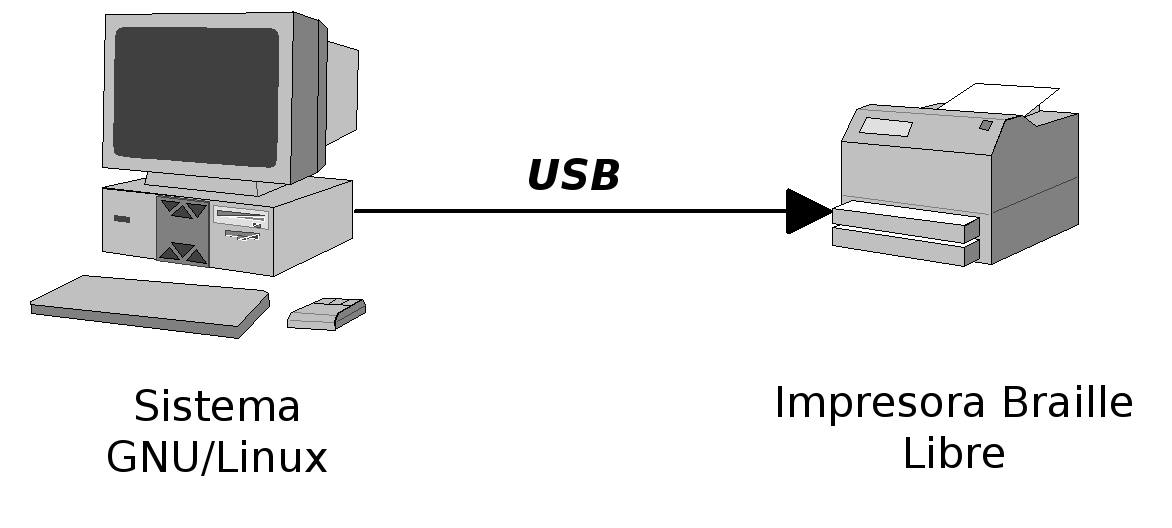
\includegraphics[scale=0.25]{./img/pc_usb_printer.png}
\caption{Clases de objetos.}
\label{fig:conexion}
\end{figure}





